\documentclass[11pt,a4paper]{article}

\usepackage{iftex}

\ifpdftex
  \usepackage[utf8]{vietnam}
  \usepackage{tgpagella}
  \usepackage{amsmath, amssymb}
\else
  \usepackage{fontspec}
  \usepackage{unicode-math}
  \setmainfont{texgyrepagella-regular.otf}[
      BoldFont = texgyrepagella-bold.otf,
      ItalicFont = texgyrepagella-italic.otf,
      BoldItalicFont = texgyrepagella-bolditalic.otf
  ]
  \setmathfont{texgyrepagella-math.otf}
  \usepackage{amsmath}
\fi

\usepackage[a4paper, margin=2.5cm]{geometry}
\usepackage{graphicx}
\graphicspath{{images/}{src/dethi/images/}{src/dethi/latex/images/}}
\usepackage{microtype}
\usepackage{titlesec}
\usepackage{enumitem}
\usepackage{tikz}
\usetikzlibrary{arrows.meta}

% Căn chỉnh khoảng cách theo chuẩn quy định
\linespread{1.05}
\setlength{\parindent}{0pt}
\setlength{\parskip}{5pt plus 2pt minus 1pt}

% Khoảng cách hiển thị công thức toán
\setlength{\abovedisplayskip}{5pt plus 2pt minus 2pt}
\setlength{\belowdisplayskip}{5pt plus 2pt minus 2pt}
\setlength{\abovedisplayshortskip}{3pt plus 1pt}
\setlength{\belowdisplayshortskip}{3pt plus 1pt}

% Định dạng tiêu đề câu hỏi
\titleformat{\section}
  {\large\bfseries}
  {\thesection}{0.5em}{}
\titlespacing*{\section}
  {0pt}{12pt plus 3pt minus 2pt}{4pt plus 1pt minus 1pt}

\pagestyle{plain}

\begin{document}

\begin{center}
    {\Large\bfseries ĐỀ THI CUỐI KỲ 20191}\\[0.2cm]
    {\bfseries MÔN THI: VẬT LÝ ĐIỆN TỬ (PH3330)}\\[0.15cm]
    \textit{Đề số 1 --- Thời gian làm bài: 90 phút}
\end{center}
\vspace{0.2cm}

%=====================================================================
% CÂU 1
%=====================================================================
\section*{Câu 1. Hiện tượng cộng hưởng từ hạt nhân}

Hãy trình bày hiện tượng cộng hưởng từ hạt nhân và nêu ứng dụng của nó.

\vspace{0.5cm}

%=====================================================================
% CÂU 2
%=====================================================================
\section*{Câu 2. Thấu kính điện tử tĩnh điện}

Một hệ quang điện tử gồm một catốt phẳng K, một lưới tăng tốc G có điện thế $U_G$ bằng $250\text{ V}$, một tấm ngăn (diapham) có điện thế $U_D$ và một anốt A được nối với diapham (Hình vẽ). Cho biết khoảng cách từ lưới tăng tốc G đến diapham D là $d_1 = 1{,}2\text{ cm}$, khoảng cách từ diapham D đến anốt A là $d_2 = 3{,}0\text{ cm}$. Xác định điện thế $U_D$ (so với catốt K) để chùm điện tử song song hội tụ lên trên anốt A.

\begin{center}
    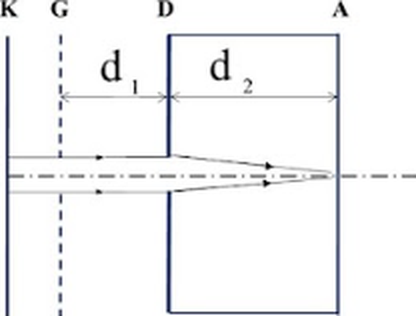
\includegraphics[height=3.4cm]{images/fig_20191.png}
\end{center}

\vspace{0.5cm}

%=====================================================================
% CÂU 3
%=====================================================================
\section*{Câu 3. Nồng độ hạt dẫn và mức Fermi trong Si}

Tính nồng độ điện tử, lỗ trống, vị trí mức Fermi của mẫu Si chứa $4{,}5 \cdot 10^{16}\text{ nguyên tử B trên } 1\text{ cm}^3$ ở nhiệt độ $300\text{ K}$. Tính giá trị của các đại lượng trên khi pha thêm vào mẫu các nguyên tử P với nồng độ $1{,}5 \cdot 10^{17}\text{ nguyên tử trên } 1\text{ cm}^3$.

Cho biết nồng độ hạt dẫn riêng trong Si ở $300\text{ K}$ là: $n_i = 1{,}45 \cdot 10^{10}\text{ cm}^{-3}$; $\Delta E_g = 1{,}12\text{ eV}$; $N_c = 2{,}8 \cdot 10^{19}\text{ cm}^{-3}$; $N_v = 1 \cdot 10^{19}\text{ cm}^{-3}$; $kT = 0{,}026\text{ eV}$.

\vspace{0.5cm}

%=====================================================================
% CÂU 4
%=====================================================================
\section*{Câu 4. Hấp thụ ánh sáng và tái hợp trong GaAs}

Một mẫu GaAs được chiếu sáng bởi ánh sáng có bước sóng $\lambda = 0{,}5\text{ }\mu\text{m}$. Công suất tia tới là $30\text{ mW}$. Nếu $1/6$ công suất đó bị phản xạ trở lại và $1/3$ thoát ra từ mặt sau của mẫu thì bề dày của mẫu bằng bao nhiêu? Tìm năng lượng nhiệt được truyền cho mạng tinh thể trong $1\text{ s}$ và số photon sinh ra do tái hợp bức xạ riêng (vùng-vùng) trong $15\text{ s}$. Biết hệ số hấp thụ $\alpha$ ứng với bước sóng trên là $4 \cdot 10^4\text{ cm}^{-1}$; $\Delta E_g = 1{,}42\text{ eV}$.

\end{document}
